\section{Results}
For the results of the experiment, each benchmark was run five times in order to achieve a more stable outcome.
The formula used for the calculation of the score per watt
can be found in the section 
\ref{sec:methodology}. \nameref{sec:methodology}.
%TODO: Das sind die Ergebnisse des Experiments, \\
%diese sind in der und der Art dargestellt, \\
%aufgefallen dabei ist, ... \\
%In Table \ref{tab:7zipBenchmarkOptiplex} ist ersichtlich ... \\


\subsection{Results of Benchmarks using 7-Zip}
The value of the Score shown in the tables of the 7-Zip benchmark is the average score the system achieved in the compression part of the benchmark.
For simplicity reasons, the scores of the decompression benchmark were not taken into account.

\begin{table} [h!]
\centering
\caption{7-Zip Benchmark Optiplex 7010}
\label{tab:7zipBenchmarkOptiplex}
\begin{tabular}{c c c c c c}
\hline
 \multicolumn{4}{|c|}{Optiplex 7010} \\   \hline
Run & Score & Watt[W] & Score/Watt[W]\\                    \hline
1 & 22502 & 136,0 &  165,5\\    
2 & 22562 & 136,4 &  165,4\\       
3 & 23431 & 137,2 &  170,8\\       
4 & 22890 & 137,6 &  166,4\\    
5 & 22071 & 137,3 &  160,8\\                                \hline
Average & 22691,2 & 136,9 & 165,8\\                      \hline
\end{tabular}
\end{table}


\begin{table} [h!]
\centering
\caption{7-Zip Benchmark Raspberry Pi 4 8GB}
\label{tab:7zipBenchmarkRaspberryPi}
\begin{tabular}{c c c c}
\hline
 \multicolumn{4}{|c|}{Raspberry Pi 4 8GB} \\            \hline
Run & Score & Watt[W] & Score/Watt[W]\\                    \hline
1 & 3841 & 10,7 &  359\\    
2 & 3963 & 10,8 &  367\\       
3 & 4018 & 10,9 &  368,6\\       
4 & 4006 & 10,9 &  367,5\\    
5 & 4007 & 11 &  364,3\\                                \hline
Average & 3967,8 & 10,86 & 365,3\\                      \hline
\end{tabular}
\end{table}









\subsection{Results of Benchmarks using Sysbench}
The scores of the Sysbench benchmark listed below are the total number of events the system achieved in the test. 

\begin{table}[h]
\centering
\caption{Sysbench Benchmark Optiplex 7010}
\label{tab:sysbenchBenchmarkOptiplex}
\begin{tabular}{c c c c}
\hline
 \multicolumn{4}{|c|}{Optiplex 7010} \\   \hline
Run & Score & Watt[W] & Score/Watt[W]\\                    \hline
1 & 67884 & 129,8 &  523\\    
2 & 67841 & 130,3 &  522,8\\       
3 & 67844 & 129,9 &  522,3\\       
4 & 67843 & 130,2 &  521,1\\    
5 & 67840 & 130,6 &  519,4\\                             \hline
Average & 67859,43 & 9,9 & 521,5\\                       \hline
\end{tabular}
\end{table}




\begin{table}[h]
\centering
\caption{Sysbench Benchmark Raspberry Pi 4 8GB}
\label{tab:sysbenchBenchmarkRaspberryPi}
\begin{tabular}{c c c c}
\hline
 \multicolumn{4}{|c|}{Raspberry Pi 4 8GB} \\            \hline
Run & Score & Watt[W] & Score/Watt[W]\\                    \hline
1 & 58543 & 9,9 &  5913,4\\    
2 & 58478 & 9,8 &  5906,9\\       
3 & 58553 & 9,9 &  5914,4\\       
4 & 58488 & 9,9 &  5907,9\\    
5 & 58495 & 9,9 &  5908,7\\                             \hline
Average & 3967,8 & 9,9 & 5910,2\\                       \hline
\end{tabular}
\end{table}


\subsection{Comparison of Results}
The results of both benchmarks show that the Raspberry Pi 4 performed significantly more energy-efficient in both tests. 
In the 7-Zip benchmark the Raspberry Pi 4 was able to achieve 2.2 times the energy efficiency of the Optiplex 7010. 
In comparison to that, the achieved score per watt of the Sysbench benchmark of the Raspberry Pi 4 was more than 11 times higher 
compared to the Optiplex 7010. 
\phantom{x}

%Barchart
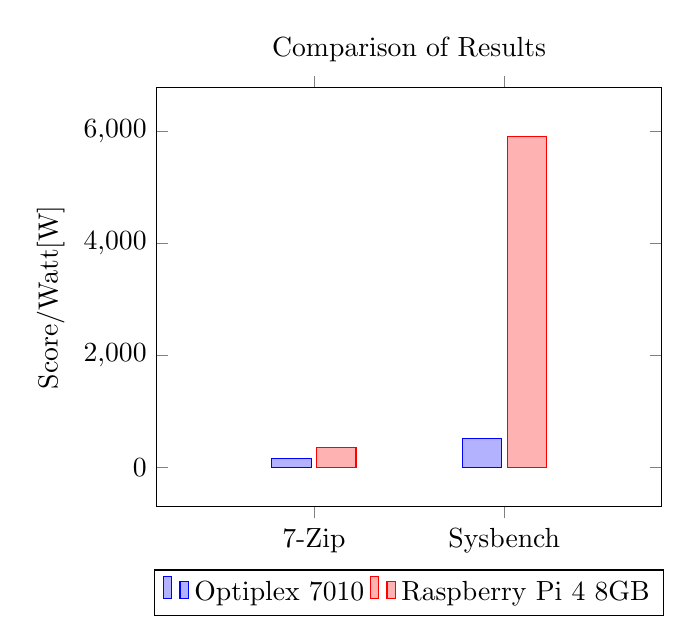
\begin{tikzpicture}
\pgfplotsset{width=8 cm}
\begin{axis}[
    ybar,
    enlargelimits=0.15,
    legend style={at={(0.5,-0.15)},
    anchor=north,legend columns=-1 align=center},
    ylabel={Score/Watt[W]},
    bar width=0.5cm,
    title= {Comparison of Results},
    symbolic x coords={7-Zip,Sysbench},
    xtick={7-Zip, Sysbench},
    enlarge x limits={abs=2cm},
]
\addplot coordinates {(7-Zip,165.8) (Sysbench,521.5)};
\addplot coordinates {(7-Zip,365.3) (Sysbench,5910.2) };

\legend{Optiplex 7010, Raspberry Pi 4 8GB}
\end{axis}
\end{tikzpicture}
